\documentclass[aspectratio=169,10pt]{beamer}
\usepackage{tikz,graphicx,booktabs}
\setbeamertemplate{navigation symbols}{}
\setbeamertemplate{footline}{}
\definecolor{ink}{HTML}{202A30}
\definecolor{muted}{HTML}{606970}
\setbeamercolor{background canvas}{bg=white}
\newcommand{\txt}[5]{\node[anchor=north west,align=left,text=#4,text width=#3 cm,inner sep=0pt,font=\fontsize{#5}{12}\selectfont] at (#1,#2)}
\newcommand{\foot}[1]{\txt{.55}{.32}{14.9}{muted}{6.5}{BioHackathon Japan 2026\hfill Asian HLA pangenome\qquad #1};}
\begin{document}
\begin{frame}[plain]
\begin{tikzpicture}[remember picture,overlay,x=1cm,y=1cm,shift={(current page.south west)}]
\txt{.55}{8.55}{14.8}{ink}{22}{Asian HLA pangenome};
\txt{.55}{7.92}{14.8}{muted}{11}{754 haplotype entries, including 462 Asian / Arab entries; 371 distinct donors};
\node[anchor=north west,inner sep=0] at (.45,7.25) {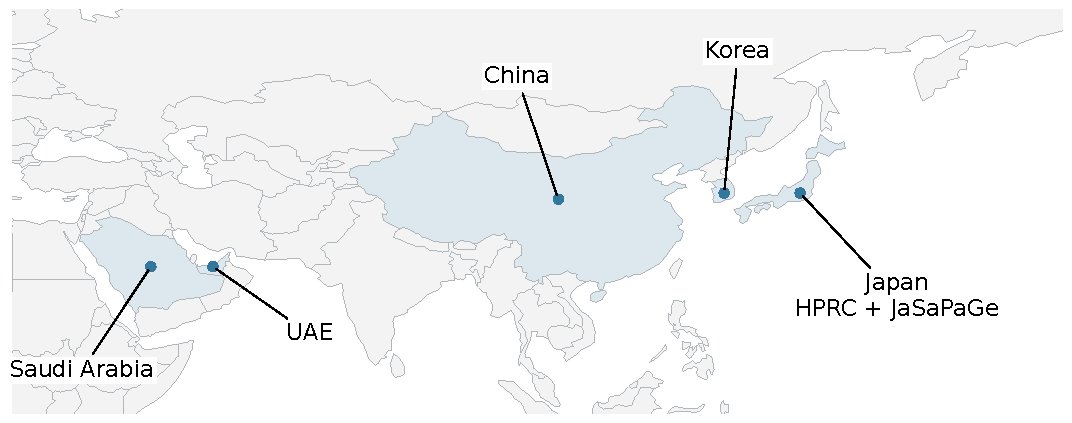
\includegraphics[width=7.5cm,height=2.8cm,keepaspectratio]{figures/paper-panels/cohort_map_hprc.pdf}};
\node[anchor=north west,inner sep=0,text=ink,font=\fontsize{8}{10}\selectfont] at (8.2,7.3) {\begin{tabular}{@{}llr@{}}\toprule
Source & Donor location & Samples\\\midrule
HPRC r2 & Worldwide, incl. Japan & 232\\
 & Japanese subset (JPT) & 16\\
APR & UAE & 53\\
JaSaPaGe & Saudi Arabia / Japan & 9 / 10\\
K-PanRef & Korea & 14\\
CPC & China & 58\\\bottomrule
\end{tabular}};
\txt{.55}{4.43}{14.8}{muted}{6.5}{HPRC includes the 16 Japanese donors. Five donors overlap between projects; GRCh38 and CHM13 add two reference haplotypes.};
\draw[black!15] (.55,4.15)--(15.4,4.15);
\txt{.55}{3.98}{8.2}{ink}{11}{MHC construction backbone};
\txt{9.05}{3.98}{6.35}{ink}{11}{Class II / DRB bundle graph};
\node[anchor=north west,inner sep=0] at (.5,3.57) {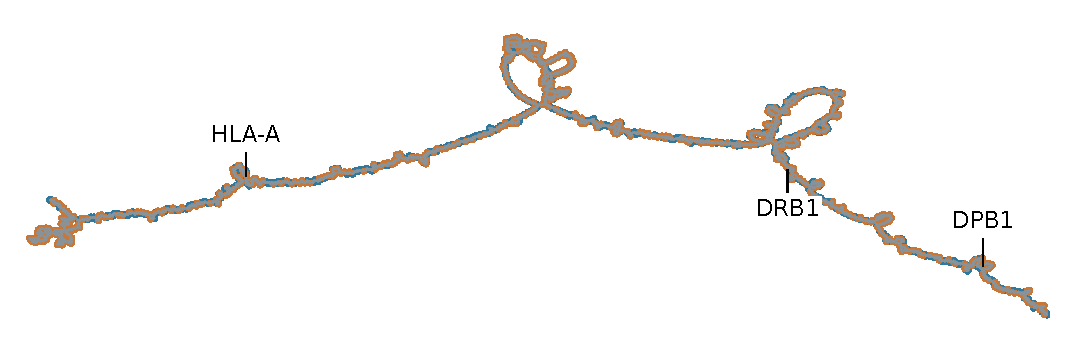
\includegraphics[width=8.45cm,height=2.65cm]{figures/paper-panels/mhc_backbone_large.pdf}};
\node[anchor=north west,inner sep=0] at (9.05,3.57) {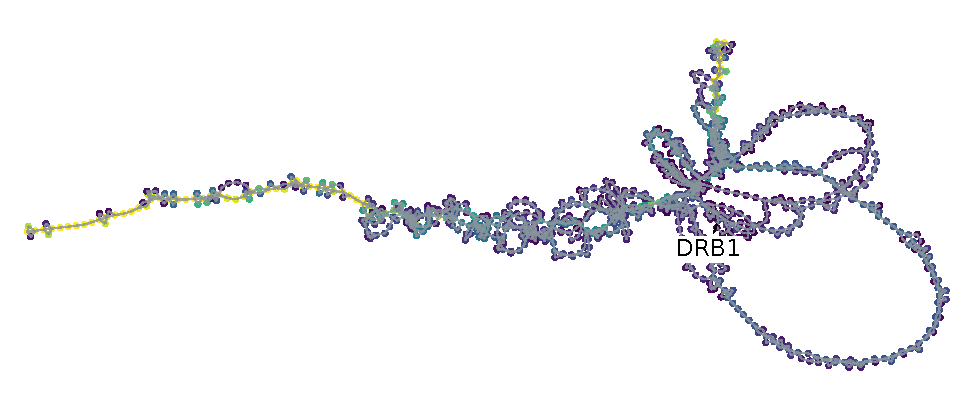
\includegraphics[width=6.35cm,height=2.65cm]{figures/paper-panels/classII_drb_large.pdf}};
\txt{.55}{.88}{8.3}{muted}{7}{1,677 segments; blue: GRCh38, orange: added sequence};
\txt{9.05}{.88}{6.4}{muted}{7}{753 haplotypes; colour: bundle sharing (purple to yellow)};
\txt{.55}{.60}{14.8}{muted}{7}{Read resource: 1000 Genomes ($n=2504$)};
\foot{1}
\end{tikzpicture}
\end{frame}
\begin{frame}[plain]
\begin{tikzpicture}[remember picture,overlay,x=1cm,y=1cm,shift={(current page.south west)}]
\txt{.55}{8.55}{14.8}{ink}{22}{Variant recovery compared with HPRC};
\txt{.55}{7.86}{14.8}{muted}{12}{Larger gains for structural variants; small changes for SNVs};
\node[anchor=north west,inner sep=0] at (.15,7.20) {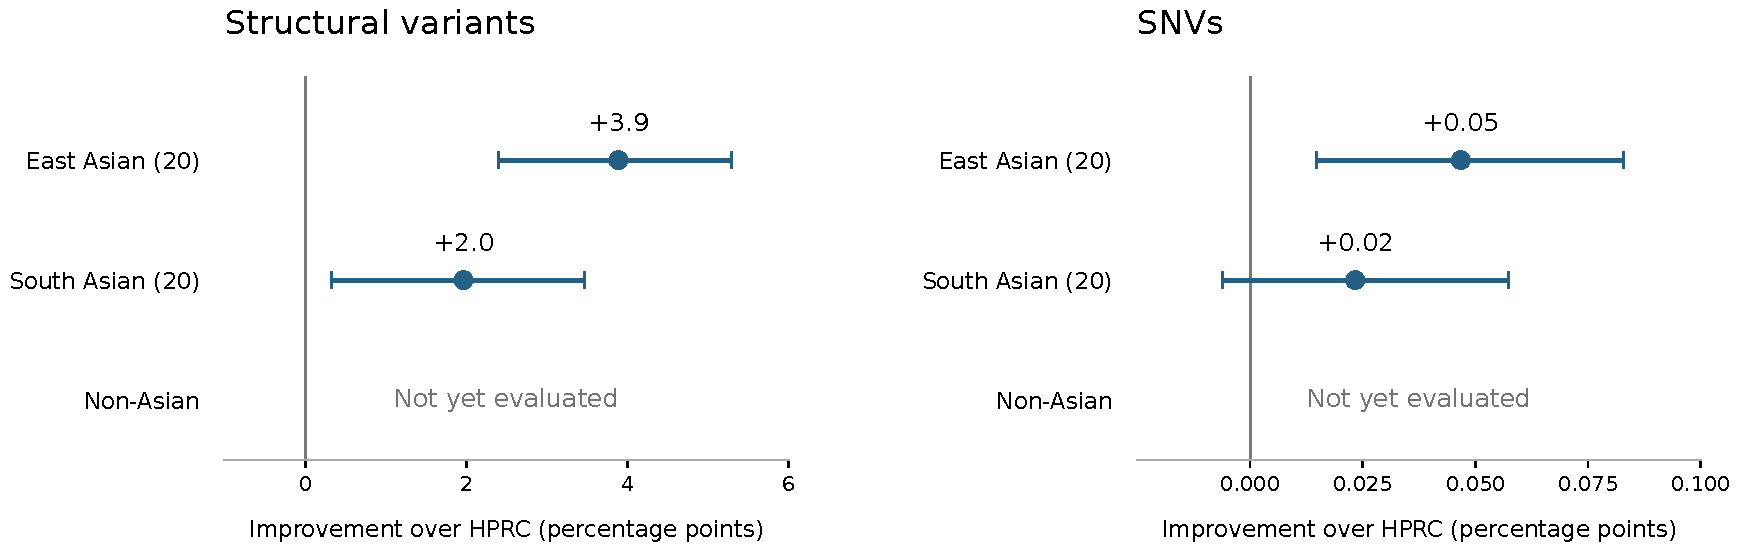
\includegraphics[width=15.55cm,height=5.5cm,keepaspectratio]{figures/paper-panels/variant_improvement.pdf}};
\txt{.65}{1.50}{14.5}{ink}{9}{Same reads and caller; expanded panel versus HPRC-only. Points: paired gains; bars: 95\% intervals.};
\txt{.65}{1.03}{14.5}{muted}{8}{SV-bearing genotypes and shared SNV sites; horizontal scales differ. Test families excluded from panels; test assemblies remain in the graph.};
\foot{2}
\end{tikzpicture}
\end{frame}
\begin{frame}[plain]
\begin{tikzpicture}[remember picture,overlay,x=1cm,y=1cm,shift={(current page.south west)}]
\node[anchor=north west,inner sep=0] at (.25,7.5) {
\includegraphics[width=5.2cm]{figures/dogohla-logo.png}};
\txt{5.8}{7.85}{9.6}{ink}{19}{T1K: independent evaluation};
\txt{5.8}{7.12}{9.6}{muted}{10}{Correct diploid HLA genotypes / eligible truth};
\node[anchor=north west,inner sep=0,text=ink,font=\fontsize{10}{14}\selectfont] at (5.8,6.4) {\begin{tabular}{@{}lrr@{}}\toprule
Truth cohort & Two fields & Four fields\\\midrule
Assembly, 64 donors & 97.2\% & 50.5\%\\
 & 495/509 & 163/323\\[10pt]
Experimental, 946 donors & 93.9\% & Unavailable\\
 & 4,437/4,723 & \\\bottomrule
\end{tabular}};
\txt{5.8}{2.95}{9.4}{muted}{9}{Assembly cohort: 16 donors each from East Asian, South Asian, European and African strata; eight HLA genes.};
\txt{5.8}{2.05}{9.4}{muted}{9}{Experimental cohort: Gourraud, five HLA genes; two-field truth only. One failed donor remains in the denominator.};
\txt{5.8}{1.10}{9.4}{muted}{8}{IPD 3.65. Failed and unresolved calls count as incorrect; eligible truth subsets differ by resolution.};
\foot{3}
\end{tikzpicture}
\end{frame}
\end{document}
